\documentclass[output=paper]{langsci/langscibook} 
 
\author{Jean Nitzke\affiliation{Johannes Gutenberg University of Mainz in Germersheim}
}
% \sectionDOI{} %will be filled in at production


\abstract{Technical developments and globalization continue to accelerate the demand for translations. To improve efficiency and cost-effectiveness, organisations increasingly resort to machine translation and edit the machine translation output to create a fluent text that adheres to the given textual conventions. This procedure is called post-editing. Usually, post-editing refers to bilingual post-editing, which means that the editor draws on the source text for the editing process. However, machine translation output can also be edited without the source text, which is referred to as monolingual post-editing.

This study analyses monolingual post-editing products and processes of 24 participants – twelve semi-professional translators and twelve professional translators. In a set of experiments they were asked to translate from scratch, post-edit and monolingually post-edit two texts per task. The quality of the product, screen-recordings and eye-tracking data obtained during research are analysed for the monolingual post-editing task. Findings show that monolingual post-editing products are of similar quality in terms of superficial errors, such as grammar, spelling, etc. compared to translations from scratch and post-edited texts. However, many more content-based errors occur. Furthermore, different patterns can be found for monolingual post-editing processes in regard to research patterns and effort compared to the other tasks.
}
\title{Monolingual post-editing: {A}n exploratory study on research behaviour and target text quality}
\rohead{Monolingual post-editing}
\maketitle
\begin{document}
 
    

% nitzke@uni-mainz.de    


\section{Introduction}

Technical development and globalization continue to increase the demand for translations. Despite economic and financial crises, more and more documents need to be translated, especially for internationally operating companies and organisations \citep{Schmitt2003, DePalma2009}. The emergence of new communication platforms – social media, discussion forums, blogs, etc. – also increases the amount of available information in various languages. To improve efficiency and cost-effectiveness, organisations increasingly resort to machine translation (MT) and edit the MT output to create a fluent text that adheres to the given textual conventions (cf. \citealt{obrien2011}; \citealt{Elsen2012}). This procedure is known as post-editing. Usually, post-editing refers to bilingual post-editing, which means that the editor draws on the source text for the editing process. Similar to translation from scratch, the post-editor needs to be fluent in source and target language. Although translation from scratch and bilingual post-editing have common characteristics, and professional translators tend to be better post-editors than untrained individuals, the tasks differ in many aspects and some additional knowledge and skills are necessary for a translator to become a successful post-editor (cf. \citealt{obrien2002}). Another possibility to edit the MT output is without the source text, which will be referred to as monolingual post-editing (MPE)\footnote{Sometimes this editing task is also referred to as \textit{blind post-editing }(e.g. \citealt{carl2013}).} here. In MPE, the editor needs only to be fluent in the target language, as the source language is of no interest. Although the post-editor merely requires knowledge of one language it does not necessarily mean that the task is simplified, because (s)he has to rely on MT output and, depending on its quality, MPE can be a difficult undertaking.


While the opinion of professional translators on MT output is very subjective, scientific papers on (bilingual) post-editing often do not take the quality of the target text into consideration at all. Therefore, the following study will look at aspects that evaluate MPE products in regard to quality and research effort. First, Section~2 provides insights on related work. \sectref{nitzke:sec:3} briefly introduces the data set, methodology, and hypothesis. In \sectref{nitzke:sec:4}, we will look at the finished MPE products and assess some error types that occurred in the target texts . Afterwards, the research effort in MPE will be analysed according to screen recording and eye-tracking data in Section~5. Research is a very time-consuming task when translating a text. Therefore, research effort should decrease in post-editing tasks. In section~6, the conclusions of the analysis will be presented and the relationship between quality and research effort will be established. The paper ends with an outlook and suggestions for future work.


\section{Related Work}

The non-scientific, professional translation community tends to have a low opinion of MT and post-editing and these topics have to be handled sensitively in this community. Some professional translators fear that their jobs are in danger, that they will be reduced to the (in some opinions less enjoyable) editing tasks, and hence they fear that the public opinion of the profession \textit{translator} will decrease (even more). However, uneducated opinions do not necessarily bear the truth and prejudice towards the technology therefore surfaces. Events such as the 20\textsuperscript{th} FIT World Congress in Berlin in July 2014 titled ``Man vs. Machine? The Future of Translators, Interpreters and Terminologists'', for example, was organised to bring translation practice and translation studies together, and to discuss the current state of MT and other technical aids including translation memory systems\footnote{Translation memory systems store translation units (usually on a sentence basis) and suggest existing translations, when the source unit is repeated in the text or another text. The translation unit does not need to be identical, usually a match of over 70\% is sufficient for the system to suggest the stored translation (these matches are called fuzzy matches and the rate, when a match is suggested, can be customised). In modern translation memory systems many features are integrated such as spell checker, concordance search, terminology management systems, etc.} that have become a necessity for professional translations over the course of the last decades. The title of the event already alludes to some of the mentioned fears of professional translators and the industry as such. Most translators, however, who have sufficient knowledge about the technical developments, probably will agree that these developments will not endanger job opportunities, but can assist the translator.



In a study conducted by the BDÜ\footnote{Bundesverband für Dolmetscher und Übersetzer -- one of the leading German professional association for Interpreters and Translators with more than 7500 members.} \citep{bdü2012}, the use of Google Translate was assessed. It was concluded that the programme might be a great online source for private communication, e.g. to make holidays preparations or as an aid while on holiday. However, for business communication, the free programme is not suitable and is very quickly stretched to its limits. The BDÜ concluded that it can be embarrassing and bad for business to send business-related e\nobreakdash-mails with mistakes or, even worse, run badly translated websites. (cf. ibid.: 9) Although the latter points are extremely valid, the study itself and the way it was conducted have to be treated very critically. Professional translators were asked to evaluate MT output for common language texts (newspaper articles about politics and menus/recipes), an excerpt of a manual belonging to a technical gadget, general terms and conditions of an online shop, and a business e\nobreakdash-mail. Although different domains were covered, only one translator evaluated each text per language combination (German into English, Spanish, Polish, and Chinese) and each domain was represented by only one text. Furthermore, the texts created by the MT system were evaluated by a pointing system that is equal to the German grading system in schools (one to six, with one being the best mark and six the worst) in the following categories: correct content, grammar, spelling, idiomacy, and overall satisfaction with the text. The grades for the MT output texts were poor for most text types - except for the category spelling. However, this method of grading the texts is very subjective and does not represent what is actually important for MT output. The question of interest should rather be: When the MT output is used in a professional environment, how much effort does it take to transform it into a reasonable target text? In the BDÜ study, post-editing was acknowledged as a necessary step to arrive at a sensible target text (cf. ibid.), but was not explained or referred to in detail. The benefits of the study are that it shows translators and potential clients that Google Translate is not almighty and that it cannot work without the help of a human translator. However, automatic translation is a rapidly developing branch and it has to be acknowledged how far the field has progressed, and that the systems do, in fact, work pretty well. Further, it should have been stated more explicitly that free online MT systems should not be compared to other MT systems, as many are far superior. Systems that are trained for one text domain and for one company will achieve much better results – assuming that they are used for the text type they were trained for: A system that was trained for household appliance manuals will probably not produce good translations for medical package inserts.



The necessity of to host events such as the FIT conference and conduct studies like the above mentioned shows that practising translators are interested in but also wary of some technical developments, and might sometimes feel threatened by automatic translation systems. Therefore, it is necessary that translation studies objectively disclose both for translators as well as for clients the abilities and limitations of MT. Publications on (bilingual) post-editing often do not take the quality of the post-editing products into account, because they are more interested in the process than in the product and product quality was not (yet) crucial for the analysis in those studies (e.g. \citet{almeida2010}; \citet{Winther2014} or \citealt{bangalore2015}). An assessment of the post-edited target text, however, would be very interesting and important in order to show the translation industry how post-editing can work and also where its limitations are. In addition, translation scholars might have a more critical and cautious attitude towards MT and the output of MT systems than computational linguists who develop the systems. While we agree that MT is better than no translation at all, MT output should not be overestimated. Scenario descriptions like the following should be treated with caution.


\begin{quotation}
``We hypothesize that for at least some language pairs, monolingual posteditors with no knowledge of the source language can successfully translate a substantial fraction of test sentences. We expect this to be the case especially when monolingual humans are domain experts with regard to the documents to be translated. If the hypothesis is confirmed, this could allow for multi-stage translation workflows, where less highly skilled monolingual posteditors triage the translation process, postediting many of the sentences, while forwarding on the most difficult sentences to more highly skilled bilingual translators.'' \citep[191]{schwartz2014}\end{quotation}

On the one hand, the quality of monolingually post-edited translation products is uncertain (unless someone who knows source and target language proof-reads the translation product). On the other hand, the more translators work on one text the more different styles get mixed and the less consistent and harder to read the text becomes. Further, translating single sentences is critical – as is suggested in the quote above that ``highly skilled bilingual translators'' (ibid.) shall take care of the more difficult sentences – because at least some inner-textual context might be necessary to translate a sentence correctly, especially when the sentence is rated as ``difficult''. It is also highly doubtful that a domain expert is cheaper than an actual bilingual translator, who is familiar with the domain. Finally, it is necessary to keep the purpose of the translation in mind, which nowadays is a prerequisite in translation studies (e.g. most famously in the Skopos theory by \citet{Vermeer1984}) and should be taken for granted for all post-editing situations as well.



A study conducted by \citet{mitchell2013} deals in part with monolingual and bilingual post-editing results (English to German/French) that are evaluated by humans. The task for the participants was to evaluate whether the monolingual/bilingual post-editing product was better, the same, or worse (per segment, not the whole text) than the MT output according to the criteria \textit{fluency}, \textit{comprehensibility}, and \textit{fidelity}. The results for the German data showed that bilingual post-editing products were improved more often (fluency 70.2\%, compr. 64\%, fidelity 56\%) than MPE products (fluency 67.3\%, compr. 57\%, fidelity 43\%). Nonetheless, the monolingual products were improved in all three criteria more often than stayed the same (fluency 20.4\%, compr. 30\%, fidelity 29\%) or became worse (fluency 12.3\%, compr. 13\%, fidelity 28\%).


\begin{quotation}
``The results of this pilot study suggest that the monolingual set-up leads to similar results in terms of improvements and degradations in fluency and comprehensibility compared to the bilingual set-up. It also leads to a greater number of improved segments for the bilingual set-up, with a considerable number of degradations, however.'' \citep[4]{mitchell2013}\end{quotation}

The group of participants was rather small and the scores of the individual participants varied a lot – especially for the German data. The same applies for the time the participants needed to edit the texts. Therefore, the study did not determine explicitly which task is more efficient and simultaneously provides the best quality. However, these initial findings are striking and it is very interesting that the participants performed so well in MPE, and that there were so many degradations of quality in the bilingual post-editing tasks.



In a study published by \citet{Koehn2010} the quality of MPE products was assessed and compared to professional translations for the languages Arabic/Chinese into English. Further, the difference between regular post-editing and interactive machine translation - different translation options were suggested by the system - was investigated. The participants could view the source text, but ``[t]he translators had no knowledge of the source script.'' (ibid.: 540) Therefore, only some indications of numbers and punctuation could be taken from the source text. The assessment was performed on sentence basis and the guideline for a correct sentence was ``a fluent translation that contains the same meaning in the document context.'' (ibid.: 541). The monolingual product was compared to a reference translation by the evaluators. Surprisingly, the professional translations were only evaluated as correct in two third of the cases, which is far less than should be expected. The monolingual post-edited sentences were correct in about one third of the cases or less: Arabic → English 35\%; Chinese → English 28\% (ibid.). These results could not be accepted for professional translations, but might be enough if the target texts were used for information gathering or similar tasks.


\section{\label{nitzke:sec:3}Data Set Description and Methodology}

The study was conducted at the University of Mainz, Department for Language, Culture and Translation Studies in Germersheim in 2012 on behalf of the Copenhagen Business School for their CRITT-TPR database \citep{carl2012critt, carl2013} which collects translation process data. In the CRITT-TPR database, data was collected for the same source texts but for different tasks, different target languages and with different tools\footnote{http://sourceforge.net/projects/tprdb/(last accessed 16\textsuperscript{th} October 2015}). Version 1.6 of the database was used for the data analysis. In the sub-project the data at hand was taken from, six texts (newspaper articles and sociology-related texts) with different complexity levels had to be processed; the source language was English and the target language was German for all texts and tasks. The lengths of the source texts vary between 100 and 148 words. In total, 24 participants took part in the English-German subset, twelve of them professional translators (university degree and some professional work experience) and twelve semi-professionals (students of the university with only little professional experience). The participants were asked to translate two texts from scratch, bilingually post-edit two machine translated texts and monolingually post-edit two machine translated texts. The texts and tasks were permuted for each translator in a way that each text was translated and bilingually/monolingually post-edited equally often. Before and after the processing task, they had to complete questionnaires, which dealt with general information about the participant, his/her attitude towards MT (in general and in regard to the machine translation output for the tasks), and self-estimation of their task performance. The MT output was produced by Google Translate (find more information on the dataset and the questionnaires in \citealt{carl2014}).


The tasks were conducted in Translog~II \citep{jakobsen2011, carl2012translog}, a programme used to record the sessions, key-strokes, mouse activity and gaze data with the help of the Tobii~TX300 eye-tracker, which also records the sessions, keystrokes, mouse activity and gaze data in Tobii Studio. There were no time restrictions and the participants could use the Internet freely as a research tool. Printed aids were not provided.



An experience vector was created to correlate research behaviour (and other phenomena) with experience. In the questionnaire prior to the experiments, the participants were asked how many years they had studied or had been studying translation at university and how many years of professional translation experience they had. This information was used and the experience vector was calculated using the following simple formula:\\

experience vector = years at university * 1 + years of professional experience * 2



As mentioned before, the participants were selected according to their status: 12 were students at the university, 12 had finished their studies and had professional work experience. However, those groups were heterogeneous in themselves: Some students already had some professional experience; some professionals had only recently completed their studies and had only little professional working experience, while other professional translators had been working as freelance translators for more than 10 years. The experience vector, therefore, represents the experience of the single participants in more detail and can be adapted for correlation calculations. The minimum value for the experience vector is two (two years at university and no professional translation experience), the maximum value is 45 (five years at university and twenty years of professional translation experience). There was no further possibility for the participants to explain what they were doing in those years of professional translation, e.g. if they were working full-time or part-time as freelance or in house translators or if they translated on a daily/regular basis, etc. Therefore, the experience vector is only the most that could be obtained from the data. It suggests that the participants gain more translation experience as practising translators than at university. The degree that students receive in Germersheim also includes linguistics and cultural studies. In addition, some courses are offered on translation theory, domain-specific knowledge or introduce scientific writing, etc. Hence, the years at university receive a lower value than years of professional experience.\footnote{The correlations in this article have been tested for different experience values as well with\par   experience vector = years at university * 1 + years of professional experience * \textbf{1}\par   experience vector = years at university * 1 + years of professional experience *\textbf{ 1.5}.\par   The correlation values and p-values naturally did change a little, but would not change the results, with only one exception in the first correlation for bilingual post-editing in section 5.1, where the p-value was already close to the critical value .05. The correlation would in this case become significant. Hence, the experience vector may need further testing with larger data sets in future work.}



The following hypotheses will be explored in the analysis. First, a difference in quality is expected (section 4): While superficial mistakes are made equally often in all three modes, content mistakes occur more often in MPE than in bilingual post-editing and translation from scratch, which would argue against MPE in professional translation tasks. Further, different Internet research patterns (section 5.1) are predicted for MPE compared to the other two tasks. Regarding production times and gaze data for research-intensive words/phrases (section 5.2), the parameters are expected to be higher in MPE than in the other tasks when research was conducted. However, the parameter should be approximately the same when the words/phrases were not researched. Finally, as neither professional nor semi-professional translators are suspected to have extensive experience with MPE and MPE is suggested to be a very different task to translation from scratch, the translation experience of the participant is expected to have no significant influence on quality and research behaviour.


\section{\label{nitzke:sec:4}Quality of the Monolingual Post-Edited Texts}

Before analysis of the Internet research instances for the MPE tasks , the quality of the final texts will be assessed. Although the notion that the post-editor does not need to know the source language to edit MT output might be very tempting for clients, the quality of MPE output is very critical, because the post-editor cannot recognise content mistakes due to the lack of a source text.


Some of the problems that occurred on various occasions in the dataset were already discussed in \citet{Culo2014}. However, different behaviour was contrasted according to the tasks and according to how different tasks influence local and global translation strategies. Single examples were discussed in regard to idiomacy, lexical consistency, word order, and preserving semantic content. While MPE performed well in the first three examples, it failed in the example of preserving semantic content. The content component is naturally essential for successful translation products and will therefore be analysed in more detail.



In \citet{Schafer2003} error categories are introduced that were established at SAP AG to develop a standard post-editing guide. At the time the paper was published, four different MT systems were used at SAP AG for different languages. The four error categories introduced are: \textit{Lexical errors}, \textit{syntactical errors}, \textit{grammatical mistakes}, and \textit{mistakes due to defective source texts}. The latter did not occur in the six source texts in this study, which needs to be a given in an experimental setting. However, this is an important aspect when technical texts are translated in practice (cf. \citealt{hornhelf1999}; \citealt{hornhelf2007}). Not only translators but also technical writers often have to deal with time-pressure and tight deadlines. Therefore, defects in the source text are quite common in technical documentation. Another aspect is that MT output was analysed in Schäfer's study, while this study will focus on mistakes in the final target texts. Therefore, syntactical mistakes were not included, because they appear less often in the post-edited text than in MT output and some syntactical structures could be categorised as bad style, which is not included in this analysis. However, a few categories have to be added, such as spelling mistakes, which occur only occasionally in MT, but quite often in human translation. Further, the key-logging system Translog~II does not include an automatic spell checker – a tool, which is standard in most of the environments that translators work in, such as word processing programmes and translation memory systems. Interestingly, especially in the other tasks (translation from scratch and bilingual post-editing) many spelling mistakes occurred, which were probably typing mistakes rather than ignorance in terms of how the word is spelled correctly. This indicates that translators tend to rely on the spell checker and are not used to focussing on these kind of mistakes.



In the first subsection, the focus will be on superficial error categories, because they can be applied for all three tasks of the study and are equally wrong in all tasks as they did not occur due to the post-editing guidelines, or resulted from the missing source text in the MPE task. The following error categories were established: \textit{Spelling},\textit{ grammar}, \textit{punctuation}, \textit{spaces}, and \textit{lexical mistakes}. The latter only concern lexical errors that can be detected without consulting the source text, which applies for the rest of the error categories as well. In general, it is expected that these superficial errors occur as often in MPE as in translation from scratch and in post-editing.



The second subsection will analyse content mistakes that occurred in MPE. This will include the following categories: \textit{Addition of information}, \textit{missing information}, and \textit{wrong information} (problematic lexical choices/content/etc.). Conclusively, those mistakes can only be discovered when the source text is taken into consideration, because a fluent text was created on the surface. Content mistakes are expected to occur much more often in the MPE task than in other tasks because of the missing source text.



The differentiation between mistakes that are obvious even without (superficial mistakes) or only with the source text (content mistakes) is essential in MPE, because the translator cannot be blamed for the content mistakes as they only result from a misinterpretation of the MT output. Superficial mistakes, however, could have been discovered or avoided. Conclusively, a high number of content mistakes in the MPE tasks argues against MPE in professional translation tasks, because they do not reflect the skills of the translator but the difficulty of the task itself.



Two of the MPE sessions had to be dismissed, because of technical problems with the key-logging software. The remaining 44 monolingual post-edited products were assessed for superficial and content mistakes. The results will be briefly compared with the results of the translation from scratch and bilingual post-editing tasks, for which 43 to 48 sessions could be assessed.


\subsection{Superficial Mistakes}

On average, the participants made 1.3 superficial mistakes (SD: 1.27) per text, which is slightly lower than for the other tasks (Translation from Scratch: Mean: 1.47, SD: 1.28; Post-Editing: Mean: 1.56, SD: 1.36). The mistakes that occurred most often were \textit{grammar} and \textit{lexical} mistakes (for both: mean:~0.48; SD: 0.76). There is no significant correlation between experience of the participants and number of mistakes\footnote{In the following correlation tests, the data are not normally distributed and hence, the non-parametric Kendall's Tau test is used.} (r\textsubscript{$\tau $}=~.01, p=~0.91). The results coincide with what was initially expected: The amount of superficial mistakes are almost the same in all three tasks. Interestingly, the experience of the participant has no influence either.

\subsection{Content Mistakes}

MPE products are suspected to be prone to content mistakes, depending on the quality of the MT output, which would be the main disadvantage in comparison to post-editing with the source text and an editor who knows the source language. In this section, we will first discuss some examples of content mistakes from the dataset and their degree of inaccuracy and then the main focus will be put on the overall dataset. Some content mistakes might originate from an incorrect MT – the mistakes were created by the MT system not the translator; the translator did not realise the mistake – while others might have arisen from a misinterpretation of MT output by the translator – the mistakes were therefore created (partly) by the translator and not (or partly) by the MT system.

\subsubsection{ Example of MPE Products with Content Mistakes}

When the content is transmitted incorrectly, the information in the text/of the communication is distorted or lost. Some content mistakes in monolingual PE were less serious than others, because they did not change the whole content of the sentences/text and did not change the overall message of the text, respectively. In the following, some examples of content mistakes in the dataset will be introduced (Table \ref{nitzke:tab:1a} \& \ref{nitzke:tab:1b}) and discussed.

\begin{table}
\begin{tabularx}{\textwidth}{lXXX} 
    & Source Sentence & Monolingual post-edited target sentence & Back-translation of target sentence \\
\lsptoprule
\multicolumn{3}{l}{Minor content mistakes}\\
(1) & All of them could be considered a burden to hospital staff. & Alle von ihnen soll er als eine Last für das Krankenhauspersonal empfunden haben. & He apparently considered all of them a burden to the hospital stuff.\\
(2) & In a gesture sure to rattle the Chinese Government, Steven Spielberg pulled out of the Beijing Olympics [\ldots]. & In einer vielbeachteten Geste reiste Steven Spielberg von den Olympischen Spielen in Peking ab [\ldots]. & In a much-noticed gesture, Steven Spielberg left the Beijing Olympics [\ldots].\\
\lspbottomrule
\end{tabularx}
\caption{Examples of Minor Content Mistakes through MPE}
\label{nitzke:tab:1a}
\end{table}



\begin{table}
\begin{tabularx}{\textwidth}{lXXX} 
    & Source Sentence & Monolingual post-edited target sentence & Back-translation of target sentence \\
\lsptoprule
(3) & China, which has extensive investments in the Sudanese oil industry, maintains close links with the Government, which includes one minister charged with crimes against humanity by the International Criminal Court in The Hague. & China, das umfangreiche Investitionen in der sudanesischen Ölindustrie getätigt hat, pflegt enge Beziehungen mit der Regierung, die auf ein Ministertreffen zum Thema Menschenrechtsverletzungen des Internationalen Strafgerichtshof in Den Haag geladen sind. & China, which has effected extensive investments in the Sudanese oil industry, maintains close links with the government, which was invited to a ministerial meeting on crimes against humanity organised by the International Criminal Court in The Hague.\\
(4) & As a result, full-time leaders, bureaucrats, or artisans are rarely supported by hunter-gatherer societies. & In Jäger-Sammler-Gesellschaften sind daher Touristen-Führer, Büroangestellte und Handwerker selten vertreten. & As a result, tourist guides, office workers, and artisans are rarely featured in hunter-gatherer societies.\\
\lspbottomrule
\end{tabularx}
\caption{Examples of Major Content Mistakes through MPE}
\label{nitzke:tab:1b}
\end{table}

The minor content mistakes do neither deliver the message of the text correctly, nor do they create a different tone in the text or drive the context in a different direction. In example (1), the perspective is wrong. The source text says that the victims of the murders could have been considered a burden to the hospital staff in general. However, the monolingual post-edited target text says that he (the murderer) considered them a burden, which is probably true as well, but is not entirely what the source text stated. In the target sentence, the second example (2) does not say that the gesture was meant to rattle the Chinese Government. So, one aspect of the source sentence is missing. However, the interpretation that the gesture was much-noticed, could be correct as well and – for what it is worth – it was probably Spielberg's intention to elicit strong reactions from the media, etc. concerning his behaviour.


The major content mistakes on the other side, deliver information that is definitely not correct. Example (3) states that the Sudanese Government was invited to a conference on crimes against humanity, while the source text actually stated that one minister of the government was charged with crimes against humanity. Therefore, the information in the target sentences is definitely incorrect and delivers the wrong, rather positive picture about the Sudanese Government. In the last example (4), the lexical miss-decisions make the target text absurd, because the target text readers would get confused as to why hunter-gatherer society should have tourist guides or clerks at all (especially as the first sentence of the text explains that hunter-gatherer societies are nomadic).


\subsubsection{Results}

On average, the participants made 2.23 (SD:~1.18) content mistakes per monolingual post-edited text, which is far more than in the other two tasks (mean:~0.46, SD:~0.71). When separated by task, there are even less content mistakes in bilingual post-editing (mean:~0.30, SD:~0.51) than in translation from scratch (mean:~0.61, SD:~0.83). One reason for this might be that the participants translate more freely in translation from scratch and therefore might transmit the information incorrectly. The mistake group that occurred most frequent in MPE was \textit{wrong information} (Mean:~1.95, SD:~1.24), while \textit{addition of information} (Mean:~0.11, SD:~0.32) and \textit{missing information }(Mean:~0.16, SD:~0.43) hardly occurred – the category \textit{wrong information }includes many more mistakes than the other two groups. Furthermore, there is no significant correlation between experience of the participants and the amount of content errors that occurred in the target texts (r\textsubscript{$\tau $}= -.06, p=~.6).

\subsection{Interpretation of Error Analysis}

The large number of content mistakes can be explained easily by the missing source text. The translator depends on the MT output and interprets it in his/her own way. They guess blindly what the correct meaning of the text might be and either they get it right or they do not. Interestingly, the participants do not get better at ``guessing'' the more translation experience they have. This also applies to superficial mistakes: Although it would have been reasonable to expect that more experienced translators make less superficial mistakes, there is no significant correlation between experience and number of mistakes. This might be explained with the help of two arguments. First, the post-editing tasks were new to most participants. Secondly, the editor in Translog~II is probably an unfamiliar work environment for professional and semi-professional participants, which was additionally not equipped with a spell checker.


The superficial errors occurred less often in MPE than in the other two tasks. One possible explanation could be that the participants were more focused on the surface of the text due to missing context. The main task in MPE is to correct and improve the text, while translation production is the main task when translating from scratch (and partly when bilingually post-editing MT output as well). Therefore, the correct transcoding of content into the target text becomes much more important in translating from scratch and bilingual post-editing. According to the key-logging data, many more tokens were typed in the translation from scratch session - on average 1117.2 tokens - while on average only 305.7 tokens were typed in the MPE task. Logically, more typing errors can occur, when more text is written.



The number of mistakes (no matter which error category) and the amount of experience do not correlate for MPE. It might be expected that the more experienced a translator is the less mistakes (s)he makes. The MPE task was (probably) very unfamiliar for all participants (the questionnaires revealed that only \textsuperscript{1}/\textsubscript{3 }of the participants had experience in bilingual post-editing), no matter how much translation experience they had. Therefore, their translation experience did not help to create a correct monolingual post-edited product. This could indicate that MPE is not (particularly) related to the task translation from scratch.


\section[Research Behaviour]{Research Behaviour}

The research the participants conducted in the MPE tasks was quite different from the other tasks, because they did not have the source text as a reference. Nonetheless, different online aids can help to improve the target texts and and/or disentangle the MT output and were used accordingly by the participants.


Due to technical problems during the recording, only 43 sessions (20 professionals and 23 semi-professionals) can be used to assess the screen recording in regard to research effort. In 51.2\% (60\% professionals, 43.5\% semi-professionals) of all MPE sessions, no Internet research was conducted at all – while no research was conducted in only 19\% (33.3\% professionals and only 4.8\% semi-professionals) of the sessions in the human translation task. Therefore, monolingual editors used Internet research far less than in other tasks, which indicates that it is a different problem they are dealing with.



The remaining sessions that contain Internet research will be analysed in the following. In the first part, the screen recording results will be assessed – How often was research necessary? What kind of sources were used? - and in the second part, the focus will be on production times and specific eye-tracking data – How long did the production of the unit take and how long was the unit looked at?


\subsection{Screen Recordings}

The Internet was consulted for research in 163 instances during all MPE sessions. On average, 3.8 research instances (SD:~5.9) were conducted per session. However, quite often one word/phrase did require more than one research instance, e.g. different online dictionaries were consulted or – especially in the MPE task – one word/phrase was first back-translated into English and then one or more of the English suggestions were looked up in the online dictionaries. Therefore, the number of problematic words/phrases that required research was much lower (mean:~1.4; SD:~2.0). Conclusively, one problematic word/phrase needed 2.7 look-up instances (SD:~4.2), which is much higher than for translation from scratch (mean:~1.5; SD:~1.2) and post-editing (mean:~1.5, SD:~1.5). This shows that the research effort per problematic word/phrase is much higher than for the other tasks, which seems reasonable, because of the missing source text. However, the values of research instances per session (TFS mean:~8, SD:~6.5; PE mean:~4.4, SD:~4.3) and problematic words/phrases per session (TFS mean:~5.3, SD:~4; PE mean:~2.8, SD:~2.6) are much lower than for the other tasks. To sum up, less research is needed for MPE, but when research is necessary, it is more elaborate.


In MPE, the correlation between experience vector and total research effort (r\textsubscript{$\tau $}=~-.17,\textsubscript{ }p=~.14) as well as the correlation between experience vector and words/phrases researched per session (r\textsubscript{$\tau $}=~-.2,\textsubscript{ }p=~.1)\footnote{In the following paragraph, the first specification in the brackets will refer to the correlation between experience vector and total research effort. The second will specify the correlation between experience vector and words/phrases researched per session.} is not significant, while the values correlate significantly for translation from scratch (r\textsubscript{$\tau $}=~-.34, p{\textgreater}~0.01/r\textsubscript{$\tau $}=~-.34, p{\textgreater}~.01) and in one case for bilingual post-editing (r\textsubscript{$\tau $}=~-.21, p=~.07/r\textsubscript{$\tau $}=~-.28, p=~.02). In both translation from scratch and bilingual post-editing, the data correlates negatively, which means that the more experience a translator has the less often (s)he researches per overall text and per word. 



Different sources were used and categorised as follows (see also \figref{nitzke:fig:1}): Bilingual dictionaries (101~instances – this group includes all sources that provide bilingual information to avoid creating too many subgroups), monolingual dictionaries (four~instances), synonym dictionaries (four instances), MT systems (18~instances), encyclopedic websites (eleven instances), search engines (21~instances), and news websites (four instances)\footnote{the three participants who used news websites did read related articles and did not find the original texts.}.




 
\begin{figure}[h]
 % TODO: replace with Nitzke1.svg
 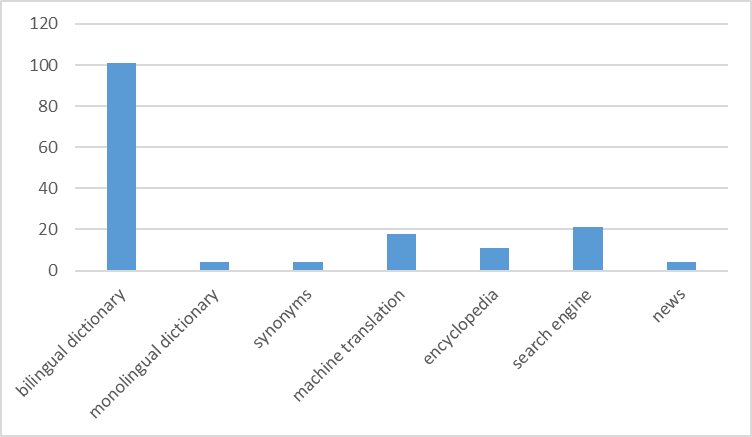
\includegraphics[width=\textwidth]{figures/Nitzke1.png}
\todo[inline]{figure should be redrawn in vector format.}
 \caption{Sources for research}
 \label{nitzke:fig:1}
\end{figure} 


In all three tasks, bilingual dictionaries were used most frequently for research. However, in MPE bilingual dictionaries were used the least often. In addition, MPE is the only task in which the translators used MT. This was caused by the missing source text, which was generated by automatic back translation of the MT output. Interestingly, all translators, who used MT as a research tool, back-translated the target text with Google Translate, although they did not know that the MT output had been originally generated by Google Translate. Maybe the back-translation would have been less helpful, if the participants had used another MT system.


\subsection{Eye-tracking Data}

The focus in this section is on the processing effort of the words/phrases that were researched most often in all tasks. The words/phrases that were researched in the Internet in at least four sessions were chosen for the analysis in order to ensure some validity. Further, some words/phrases were excluded for different reasons, e.g. last words of headlines, because some gaze data may have been assigned to the last words of the headline although the gaze was somewhere else in the  rest of the line after the line break. Words/phrases that occurred more than once in the text were excluded as well, because it cannot be determined for certain, where in the text the word/phrase became problematic. After excluding these research instances, a total of 28 words/phrases can be analysed.


However, as already discussed in section 5.1, there was less research in MPE than in bilingual post-editing and translation from scratch. Conclusively, some of the words/phrases were not researched in MPE and will be excluded as well. Finally, one word had to be excluded due to technical problems in the eye-tracking data (see \tabref{nitzke:tab:2} for the amount of remaining words per text). 

\begin{table}
\begin{tabular}{lrrrrrr} & Text 1 & Text 2 & Text 3 & Text 4 & Text 5 & Text 6\\
\lsptoprule
No. Words/Phrases & 0 & 2 & 3 & 1 & 3 & 2\\
\lspbottomrule
\end{tabular}
\caption{Number of words/phrases that were taken into consideration per text, excluding those that were not researched in monolingual editing.}
\label{nitzke:tab:2}
\end{table}



In two instances, the word/phrase was not researched during bilingual post-editing either, e.g. ``insistence'' in text two was looked up five times in the translation from scratch session, but never in the post-editing sessions. The machine translated ``insistence'' with ``Beharren'' which is an acceptable translation for the word in the context of text two and therefore reduced the research effort in the post-editing tasks. Conclusively, the MT system made the translation process in those instances easier, because it was a high research effort word in the translation from scratch task, but did not have to be researched when the text was machine translated.



When phrases were looked up, the gaze data for the whole phrase was taken into consideration and not only for the words that were actually looked up. For example, in the dependent sentence ``which includes one minister charged with crimes against humanity by the International Criminal Court in The Hague'' some translators researched ``Criminal Court'', ``International Criminal Court'', ``International Criminal Court in The Hague'', etc. The production time and gaze data of the whole phrase ``International Criminal Court in The Hague'' was taken into consideration, even if only ``Criminal Court'' was looked up, so that the different research instances are comparable, no matter how the translator decided to gather information on the phrase.



The CRITT-TPR database contains tables with key-logging and eye-tracking data for each translator and task (see \citealt{carl2013} for a detailed explanation of the various parameters). To compare the data, two parameters were chosen, one concerned with production time (\textit{Dur}) and one with gaze data (\textit{GazeT}):


\begin{quotation}
 \textbf{Dur}: Duration of unit production time [\ldots]\\
  \textbf{GazeT}: Total gaze time on target text unit [\ldots] (ibid.: 22) 
\end{quotation}

Dur and GazeT include all instances in which the target word/phrase was produced or looked at. Therefore, they can be used to compare the mental effort of the particular unit in the overall session. This is important because the word/phrase may not have been considered problematic at first glance. Nor can it be implied that the word/phrase became unproblematic after the research instance or the (first) production of the target word/phrase. In future analyses of the translation from scratch and bilingual post-editing task, the parameter for the gaze on the source text will be taken into consideration as well. However, as the source text is missing in this task, data on the source text will obviously not be taken into account.

% table before
% \begin{table}
% \begin{tabularx}{\textwidth}{lXXXXX}
% \lsptoprule
% Words/phrases & 
% % \rotatehead{Total amount of sessions (MPE sessions)} & 
% \rotatehead[2cm]{\mbox{Sessions (MPE sessions)}} & 
% % \rotatehead{Total amount of sessions with research on the word/phrase} &
% \rotatehead[2cm]{\mbox{Sessions with research} \mbox{on the word/phrase}} &
% % \rotatehead{Total amount of sessions with no research} & 
% \rotatehead[2cm]{\mbox{Sessions with no research}} & 
% % \rotatehead{Total amount of sessions with research in MPE (n)} & 
% \rotatehead[2cm]{\mbox{Sessions with} \mbox{ research in MPE (n)}} & 
% % \rotatehead{Total amount of sessions with no research in MPE}\\
% \rotatehead[3cm]{\mbox{Sessions with no } \mbox{research in MPE}}\\
% \midrule
% below-inflation & 20 (7) & 5 & 15 & 1 & 6\\
% cut interest rates & 20 (7) & 7 & 13 & 2 & 5\\
% rattle & 21 (7) & 11 & 10 & 2 & 5\\
% halt & 21 (7) & 5 & 16 & 1 & 6\\
% Khartoum & 21 (7) & 6 & 15 & 1 & 6\\
% incentives & 22 (7) & 10 & 12 & 2 & 5\\
% associate & 21 (8) & 10 & 11 & 2 & 6\\
% exposure & 21 (8) & 9 & 12 & 4 & 4\\
% bureaucrats & 21 (7) & 9 & 12 & 4 & 3\\
% full-time leader & 21 (7) & 8 & 13 & 2 & 5\\
% \lspbottomrule
% \end{tabularx}
% \caption{Occurrences of the most researched words/phrases in the complete dataset and in MPE}
% \todo[inline]{Suggest splitting table into two with columns [1,2,3,4] and [1,2,5,6]. Content of column 2 would be split as well. OK?}
% \label{nitzke:tab:3}
% \end{table}

% split table
% part 1
\begin{table}
\begin{tabularx}{\textwidth}{lXXXXX}
\lsptoprule
Words/phrases & 
% \rotatehead{Total amount of sessions (MPE sessions)} & 
\rotatehead[3cm]{\mbox{Sessions (MPE sessions)}} & 
% \rotatehead{Total amount of sessions with research on the word/phrase} &
\rotatehead[3cm]{\mbox{Sessions with research} \mbox{on the word/phrase}} &
% \rotatehead{Total amount of sessions with no research} & 
\rotatehead[3cm]{\mbox{Sessions with no research}}\\
\midrule
below-inflation & 20 (7) & 5 & 15 \\
cut interest rates & 20 (7) & 7 & 13 \\
rattle & 21 (7) & 11 & 10 \\
halt & 21 (7) & 5 & 16 \\
Khartoum & 21 (7) & 6 & 15 \\
incentives & 22 (7) & 10 & 12 \\
associate & 21 (8) & 10 & 11 \\
exposure & 21 (8) & 9 & 12 \\
bureaucrats & 21 (7) & 9 & 12 \\
full-time leader & 21 (7) & 8 & 13 \\
\lspbottomrule
\end{tabularx}
\caption{Occurrences of the most researched words/phrases in the complete dataset and in MPE}
\label{nitzke:tab:3a}
\end{table}

% part2
\begin{table}
\begin{tabularx}{\textwidth}{lXXXXX}
\lsptoprule
Words/phrases & 
% \rotatehead{Total amount of sessions (MPE sessions)} & 
\rotatehead[2cm]{\mbox{Sessions (MPE sessions)}} & 
% \rotatehead{Total amount of sessions with research in MPE (n)} & 
\rotatehead[2cm]{\mbox{Sessions with} \mbox{ research in MPE (n)}} & 
% \rotatehead{Total amount of sessions with no research in MPE}\\
\rotatehead[3cm]{\mbox{Sessions with no } \mbox{research in MPE}}\\
\midrule
below-inflation & 20 (7) & 1 & 6\\
cut interest rates & 20 (7) & 2 & 5\\
rattle & 21 (7) & 2 & 5\\
halt & 21 (7) & 1 & 6\\
Khartoum & 21 (7) & 1 & 6\\
incentives & 22 (7) & 2 & 5\\
associate & 21 (8) & 2 & 6\\
exposure & 21 (8) & 4 & 4\\
bureaucrats & 21 (7) & 4 & 3\\
full-time leader & 21 (7) & 2 & 5\\
\lspbottomrule
\end{tabularx}
\caption{Occurrences of the most researched words/phrases in the complete dataset and in MPE}
\label{nitzke:tab:3b}
\end{table}

The mean values for Dur (\tabref{nitzke:tab:4}) and GazeT (\tabref{nitzke:tab:5}) will be compared for the whole dataset with the MPE data in the next paragraphs. No statistical evaluation will be conducted for the data, because n is very small for the research instances per word/phrase task (see Table \ref{nitzke:tab:3a} and \ref{nitzke:tab:3b}). In a follow-up study the number of participants would have to be increased to find statistically significant differences between the different tasks. It is expected that \textit{Dur }and\textit{ GazeT }are higher for researched words/phrases in MPE than the other tasks. The parameter should be approximately the same when the words/phrases were not researched.

% original table (not transposed)
% \begin{table}
% \begin{tabularx}{\textwidth}{XXXXXXXXXXX}
% \lsptoprule
% Dur & 
% \rotatehead[3cm]{below-inflation} & 
% \rotatehead[3cm]{cut interest rates} & 
% \rotatehead[3cm]{rattle} & 
% \rotatehead[3cm]{halt} & 
% \rotatehead[3cm]{Khartoum} & 
% \rotatehead[3cm]{incentives} & 
% \rotatehead[3cm]{associate} & 
% \rotatehead[3cm]{exposure} & 
% \rotatehead[3cm]{bureaucrats} & 
% \rotatehead[3cm]{full-time leader}\\
% \midrule
% All research & 7369.2 & 8622.6 & 10796.5 & 10421.2 & 13478.8 & 2756.8 & 1753.5 & 9798.3 & 1015.7 & 20733.8\\
% All Non-research & 5114.9 & 1400.8 & 2817.7 & 940.9 & 3330.8 & 5712.2 & 777.6 & 193.8 & 1281.6 & 3884.3\\
% MPE research & 8533 & 1069 & 5070.5 & 42869 & 14291 & 4867 & 876 & 24008.5 & 1336.3 & 2160.5\\
% MPE Non-research & 3737.3 & 1227 & 3975 & 235.5 & 215 & 2851 & 383 & 0 & 0 & 2764.2\\
% \lspbottomrule
% \end{tabularx}
% \caption{Mean Dur for the particular word/phrase for all research instances, all non-research instances, MPE research, and MPE research}
% \todo[inline]{suggest swapping rows and columns for this table}
% \label{nitzke:tab:4}
% \end{table}

\begin{table}
\begin{tabularx}{\textwidth}{XXXXX}
\lsptoprule
Dur &
\rotatehead[2cm]{All research} & 
\rotatehead[2cm]{All Non-research} & 
\rotatehead[2cm]{MPE research} & 
\rotatehead[2cm]{MPE Non-research} \\
\midrule
below-inflation & 7369.2  & 5114.9  & 8533  & 3737.3  \\ 
cut interest rates & 8622.6  &  1400.8  &  1069  &  1227  \\ 
rattle & 10796.5  &  2817.7  &  5070.5  &  3975  \\ 
halt & 10421.2  &  940.9  &  42869  &  235.5  \\ 
Khartoum & 13478.8  &  3330.8  &  14291  &  215 \\ 
incentives & 2756.8  &  5712.2  &  4867  &  2851  \\ 
associate & 1753.5  &  777.6  &  876  &  383  \\ 
exposure & 9798.3  &  193.8  &  24008.5  &  0  \\ 
bureaucrats & 1015.7  &  1281.6  &  1336.3  &  0  \\ 
full-time leader & 20733.8 &  3884.3 &  2160.5  &  2764.2  \\ 
\lspbottomrule
\end{tabularx}
\caption{Mean Dur for the particular word/phrase for all research instances, all non-research instances, MPE research, and MPE research}
\label{nitzke:tab:4}
\end{table}

In six out of ten instances, the mean for the production of the word/phrase is higher in MPE than the mean duration for all tasks, when the word/phrase was researched. The mean duration for MPE is only higher in one instance than in all tasks, when the word/phrase was not researched. These results were expected and indicate that the production time for research intensive words/phrases is higher in MPE than in other tasks. One reason could be that, in general, the MT output first has to be deleted in post-editing and then the new translation is inserted, while there is only the production of the word/phrase in translation from scratch. Further, due to the missing source text, the translator might be insecure with his/her solution and therefore needs more time to produce the unit than in bilingual post-editing. To prove these hypotheses, more research instances and hence more participants would be necessary.

% original table (not transposed)
% \begin{table}
% \begin{tabularx}{\textwidth}{XXXXXXXXXXX}
% \lsptoprule
% 
% GazeT &
% \rotatehead[3cm]{below-inflation} & 
% \rotatehead[3cm]{cut interest rates} & 
% \rotatehead[3cm]{rattle} & 
% \rotatehead[3cm]{halt} & 
% \rotatehead[3cm]{Khartoum} & 
% \rotatehead[3cm]{incentives} & 
% \rotatehead[3cm]{associate} & 
% \rotatehead[3cm]{exposure} & 
% \rotatehead[3cm]{bureaucrats} & 
% \rotatehead[3cm]{full-time leader}\\
% \midrule
% All research & 2671.6 & 7395.9 & 14353.5 & 7217.6 & 2330.5 & 2484 & 1578.1 & 2759.3 & 11018.7 & 6062.9\\
% All Non-research & 10123 & 5431.9 & 4764.1 & 2052.5 & 1329.6 & 4388.3 & 2256.5 & 2943.2 & 5249.2 & 7167.8\\
% MPE research & 2160 & 3797.5 & 1455 & 1325 & 1634 & 406.5 & 3221.5 & 1067.5 & 14563 & 3178\\
% MPE Non-research & 8775.7 & 3659 & 1083.8 & 1657.5 & 158.3 & 1398.2 & 1706.7 & 424.8 & 6288.7 & 7814.4\\
% \lspbottomrule
% \end{tabularx}
% \caption{Mean GazeT for the particular word/phrase for all research instances, all non-research instances, MPE research, and MPE research}
% \todo[inline]{suggest swapping rows and columns for this table}
% \label{nitzke:tab:5}
% \end{table}

\begin{table}
\begin{tabularx}{\textwidth}{XXXXX}
\lsptoprule

GazeT &
\rotatehead[2cm]{All research} &
\rotatehead[2cm]{All Non-research} &
\rotatehead[2cm]{MPE research} &
\rotatehead[2cm]{MPE Non-research} \\
\midrule
below-inflation & 2671.6  & 10123  & 2160  & 8775.7  \\ 
cut interest rates & 7395.9  &  5431.9  &  3797.5  & 3659  \\ 
rattle & 14353.5  &  4764.1  &  1455  &  1083.8  \\ 
halt & 7217.6  &  2052.5  &  1325  &  1657.5  \\ 
Khartoum & 2330.5  &  1329.6  &  1634  &  158.3  \\ 
incentives & 2484  &  4388.3  &  406.5  &  1398.2  \\ 
associate & 1578.1  &  2256.5  &  3221.5  &  1706.7  \\ 
exposure & 2759.3  &  2943.2  &  1067.5  &  424.8  \\ 
bureaucrats & 11018.7  &  5249.2  &  14563  &  6288.7  \\ 
full-time leader & 6062.9 &  7167.8 &  3178 &  7814.4  \\ 
\lspbottomrule
\end{tabularx}
\caption{Mean GazeT for the particular word/phrase for all research instances, all non-research instances, MPE research, and MPE research}
\label{nitzke:tab:5}
\end{table}


The mean for GazeT of the word/phrase is higher in MPE than the mean duration for all tasks in two out of ten instances. This is true for both cases when the word/phrase was researched and when it was not. This means that more gaze is spent in only 20\% of the research-intensive words/phrases, no matter whether the word/phrase was researched in the Internet or not. Therefore, the processing of research-intensive words/phrases seems to be equally or even less problematic than in other tasks, which is contrary to what was expected. Especially, when we take into consideration that processing also takes place while reading the source text in translations from scratch and bilingual post-editing. As mentioned above, n for research instances in MPE is too small to conduct any valuable significance tests. Hence, the discussed results indicate a tendency, but a much larger dataset would be needed to test the hypothesis accordingly.


\section{Conclusion}

The quality of MPE products is not comparable to translations from scratch or bilingual post-edited texts. While the surface of the text is good and even fewer superficial mistakes occurred in MPE than in other tasks of the dataset, the content of the products is error-prone and is not acceptable. The target texts often contain (slightly) different meanings than the source texts and are therefore not suitable for many translation purposes, especially if the translation is intended for publication. For information gathering, however, the target texts could be used in most cases.


Research behaviour in MPE is different than in other tasks. No internet research was used at all in over half of the sessions. In those sessions that contained Internet research, less words/phrases were researched. However, when research is necessary, it is more elaborate, because the participants use more research instances to find a solution for a difficult word/phrase. The main sources of research were bilingual dictionaries in MPE as well as in the other tasks. However, in relation to other sources, it was used less frequently. Further, only monolingual editors used MT systems as a resource to create a source-text-like text.



The production times of research intensive words tend to be higher in MPE than in other tasks. Contrary to what was expected, the eye-tracking data for MPE do not indicate more gaze behaviour than in other tasks. However, the dataset is too small to draw any statistically significant solutions.



There is no statistically significant correlation between experience and research behaviour. That might indicate that MPE is only partly related to translation and that translators do not benefit much from their translation experience. Making sense out of an error-prone text that may or may not be the correct interpretation, due to lacking reference material (in regular translation situations the source text) is not what translators are trained to do, which was also indicated in the retrospective questionnaire.



In the retrospective questionnaire, we asked the participant how satisfied they had been with their post-editing tasks. The participants could choose from five answers, each choice was given a value that will be added in brackets – highly satisfied (two points), somewhat satisfied (one point), neutral (no point), somewhat dissatisfied (minus one point) and highly dissatisfied (minus two points). The mean of the added values indicates which tendency the participants had in judging their results. The professionals were quite critical about their work and were not satisfied (mean:~-0.68, SD:~1.43) with their monolingual post-edited target texts. The semi-professionals were neither satisfied nor dissatisfied with their work (mean:~0.08, SD:~1.08). The satisfaction with the bilingual post-editing task was higher, however professionals (mean:~0.18, SD:~1.25) were still more critical about their bilingual post-editing product than semi-professionals (mean:~0.67, SD: 0.89). This low satisfaction with the MPE tasks could be a sign that the participants were rather frustrated with the task. The task was new to (most of) the participants and they could not use the problem-solving strategies they use in translation from scratch. One remaining question is how much influence experience in MPE would have on the final target text. Maybe some strategies that are unique for MPE would be developed after some experience and the task would a) produce better target texts and b) would be less exhausting/frustrating.


\section{Future Work and Outlook}

Unfortunately, the questionnaires did not include questions about the translators' proof-reading experience. Usually, translators have to proof-read other translation products or regular texts quite often, but some (professional) translators might do proof-reading as one of their main work task, while others might just do it occasionally. Semi-professional translators might have different experience in proof-reading as well. For bilingual post-editing, it has already been agreed that it is more than mere proof-reading of MT output (e.g. \citealt{obrien2002}). However, due to the lack of a source text monolingual post-editing might be closer to traditional reviewing/proof-reading than bilingual post-editing, even if the MT system often produces completely different mistakes and makes more mistakes than a human translator would. Therefore, there might be a significant correlation between revising/poof-reading experience and MPE, which could be explored in a follow-up study.


The amount of data in this study is critical to explore research behaviour and research patterns that are different to those in bilingual post-editing and translation from scratch. In particular, there was far too little eye-tracking data to draw significant conclusions on likeliness or differences between the different tasks. A group of 24 participants is as such a small group. Additionally, every participant monolingually edited only every third text and not every participant looked up the same words/phrases. Therefore, a much bigger group would be necessary to evaluate significant relations.



Research behaviour in MPE should also be investigated for other text types, as translating newspaper articles and other texts in general language is not common in professional translation practice. An online survey \citep{Hommerich2011} conducted by the BDÜ reported that 49\% of the members that participated in the study (in total 1570) specialised in the field ``Industry and Technology (general)'', 45\% in ``Law and Administration'', 41\% in ``Economics, Trade, and Finances``, 25\% in ``Medicine and Pharmacy'', and 23\% in ``Information Technology''. Only few translators specialised in fields that might require the use of general language like ``Culture and Education'' (13\%), ``Sports, Recreation, and Tourism'' (10\%), or ``Media and Art'' (9\%) - though most of these fields might require domain-specific language and terminology as well. As a consequence, the results of domain-trained MT systems would probably be of better quality than the MT output of Google Translate.



MPE is a noble goal for MT. The notion that the user does not need to know the source language and that only a few corrections concerning grammar and syntax are necessary to create a functioning text is very appealing, but from a translation studies perspective this will not become a reality in the near future. Of course, the success of MT output is extremely dependent on the the purpose of the target text. When the text is intended for publication, a source text will be necessary for the translator to ensure that the content of the target text is correct. In stylistically diverse texts, translation from scratch might still be preferable to post-editing, but even in domain-specific texts which would be proof-read by monolingual domain experts, the risk of material or personal damage is too high to not consider the source text. Nonetheless, MPE is a task that will remain interesting in research, e.g. to evaluate MT output.



In the future, MT output might become so accurate that MPE becomes an option for professional translation tasks. As soon as this goal is achieved – at least for some translation purposes – it would be reasonable to consider integrating MPE into translation training in a similar way to bilingual post-editing \citep{obrien2002}, because the data indicate the the task is very different from translation from scratch and bilingual post-editing. However, bilingual post-editing needs to be integrated into university curricula first. Bilingual post-editing courses also have the advantage that students might become aware of the dangers and difficulties of MPE by themselves or might be made aware of these by the instructor, so that they can make the right decisions if they ever encounter a MPE job and can consult clients in regard to the MPE task.


% \section[References]{References}
% 
% Almeida, Giselle de, and Sharon O’Brien. 2010. “Analysing Post-Editing Performance: Correlations with Years of Translation Experience.” In \textit{EAMT 2010: Proceedings of the 14th Annual Conference of the European Association for Machine Translation}. Saint-Raphaël, France.
% 
% 
% 
% Bangalore, Srinivas, Bergljot Behrens, Michael Carl, Maheshwar Gankhot, Arndt Heilmann, Jean Nitzke, Moritz Schaeffer, and Annegret Sturm. 2015. “The Role of Syntactic Variation in Translation and Post-Editing.” \textit{Translation Spaces} 4 (1): 119–44.
% 
% 
% 
% BDÜ. 2012. \textit{Mensch ./. Maschine - Ergebnisse Der BDÜ-Untersuchung Zur Qualität Der Übersetzungen Durch Google Translate}. Pressedossier. Berlin: BDÜ.
% 
% 
% 
% Carl, Michael. 2012a. “The CRITT TPR-DB 1.0: A Database for Empirical Human Translation Process Research.” In \textit{Proceedings of the AMTA 2012 Workshop on Post-Editing Technology and Practice (WPTP 2012)}, 9–18.
% 
% 
% 
% ———. 2012b. “Translog-II: A Program for Recording User Activity Data for Empirical Translation Process Research.” In \textit{Proceedings of The Eighth International Conference on Language Resources and Evaluation}. Istanbul, Turkey.
% 
% 
% 
% Carl, Michael, and Moritz J Schaeffer. 2013. “The CRITT Translation Process Research Database V1. 4.”
% 
% 
% 
% Carl, Michael, Silke Gutermuth, and Silvia Hansen-Schirra. 2014. “Post-Editing Machine Translation–a Usability Test for Professional Translation Settings.” \textit{Psycholinguistic and Cognitive Inquiries in Translation and Interpretation Studies. Newcastle upon Tyne: Cambridge Scholars Publishing}.
% 
% 
% 
% Čulo, Oliver, Silke Gutermuth, Silvia Hansen-Schirra, and Jean Nitzke. 2014. “The Influence of Post-Editing on Translation Strategies.” In \textit{Post-Editing of Machine Translation: Processes and Applications}. Newcastle upon Tyne: Cambridge Scholars Publishing.
% 
% 
% 
% DePalma, Donald A. 2009. “Chancen Der Globalisierung.” \textit{MDÜ}, no. 2/09: 10–13.
% 
% 
% 
% Elsen, Harald. 2012. “Postediting - Schreckgespenst Oder Perspektive.” \textit{MDÜ}.
% 
% 
% 
% Hommerich, Christoph, and Nicole Reiß. 2011. “Ergebnisse Der BDÜ-Mitgliederbefragung.”
% 
% 
% 
% Horn-Helf, Brigitte. 1999. \textit{Technisches Übersetzen in Theorie Und Praxis}. Francke.
% 
% 
% 
% ———. 2007. \textit{Kulturdifferenz in Fachtextsortenkonventionen: Analyse Und Translation: Ein Lehr-Und Arbeitsbuch}. Vol. 4. Peter Lang.
% 
% 
% 
% Jakobsen, Arnt Lykke. 2011. “Tracking Translators’ Keystrokes and Eye Movements with Translog.” \textit{Methods and Strategies of Process Research}, 37–55.
% 
% 
% 
% Koehn, Philipp. 2010. “Enabling Monolingual Translators: Post-Editing vs. Options.” In \textit{Human Language Technologies: The 2010 Annual Conference of the North American Chapter of the Association for Computational Linguistics}, 537–45. Association for Computational Linguistics.
% 
% 
% 
% Mitchell, Linda, Johann Roturier, and Sharon O’Brien. 2013. “Community-Based Post-Editing of Machine-Translated Content: Monolingual vs. Bilingual.”
% 
% 
% 
% O’Brien, Sharon. 2002. “Teaching Post-Editing: A Proposal for Course Content.” In \textit{Sixth EAMT Workshop}, 99–106. Manchester, U.K. http://www.mt-archive.info/EAMT-2002-OBrien.pdf.
% 
% 
% 
% O’Brien, Sharon. 2011. “Towards Predicting Post-Editing Productivity.” \textit{Machine Translation} 25 (3): 197–215. doi:10.1007/s10590-011-9096-7.
% 
% 
% 
% Reiß, Katharina, and Hans J. Vermeer. 1984. \textit{Grundlegung einer allgemeinen Translationstheorie}. Linguistische Arbeiten 147. Tübingen: Niemeyer. http://openlibrary.org/b/OL2946081M/Grundlegung\_einer\_allgemeinen\_Translationstheorie.
% 
% 
% 
% Schäfer, Falko. 2003. “MT Post-Editing: How to Shed Light on the ‘unknown Task’. Experiences at SAP.” In \textit{Controlled Language Translation}, 133–40. Dublin, Ireland.
% 
% 
% 
% Schmitt, Peter A. 2003. “Berufsbild.” In \textit{Handbuch Translation}, 2nd ed., 1–5. Tübingen: Stauffenburg.
% 
% 
% 
% Schwartz, Lane OB, Timothy Anderson, Jeremy Gwinnup, and Katherine M Young. 2014. “Machine Translation and Monolingual Postediting: The Afrl Wmt-14 System.” In \textit{Proceedings of the Ninth Workshop on Statistical Machine Translation}, 186–94.
% 
% 
% 
% Winther Balling, Laura, and Michael Carl. 2014. “Production Time Across Languages and Tasks: A Large-Scale Analysis Using the CRITT Translation Process Database.” \textit{Psycholinguistic and Cognitive Inquiries in Translation and Interpretation Studies. Newcastle upon Tyne: Cambridge Scholars Publishing}.



%\subsection*{Abbreviations}
%\subsection*{Acknowledgements}

\printbibliography[heading=subbibliography,notkeyword=this]

\end{document}